\begin{section}{Some Attacks on Hash Based Signatures}


This section examines some attacks on hash-based signature algorithms.

\subsection{Intermediate Value Guessing Attack}

This attack was defined in the paper by Booth et al.\cite{booth2021intermediate}. In the document by Hülsing et al. \cite{huelsing2018rfc}, it is stated that the secret key values used in the WOTS+ signature must be generated in a uniformly distributed , but the method is left to the implementer. Assume that the WOTS+ secret keys (\texttt{osk}) are generated from the seed values \texttt{seed\textsubscript{OTS},i} as follows:

\[
\texttt{osk} = (x_{i,1}, x_{i,2}, \ldots, x_{i,l}) = (F(\texttt{seed}_{\text{OTS},i},1), \ldots, F(\texttt{seed}_{\text{OTS},i},l))
\]

Under this assumption:

\begin{itemize}
    \item The signatures of messages whose base-$w$ representation includes zero values leak the corresponding indices of \texttt{osk}. For instance, if the base-$w$ representation of message $M$ is $BM = (b_1, 0, b_2)$, then the signature $\sigma_M = (Z_1, x_{i,2}, Z_3)$ reveals $x_{i,2}$. (Here, each $Z$ value is derived by applying the hash algorithm to a secret key index $w$ times.)
    
    \item The \texttt{osk} values used to sign different messages are generated from different seed values.
    
    \item Using a different seed for each WOTS+ secret key allows a multi-target attack, as described below.
\end{itemize}

In this attack, the adversary proceeds as follows:

\begin{itemize}
    \item Executes the signing oracle to obtain multiple WOTS+ message-signature pairs.
    \item Filters out pairs where fewer than two \texttt{osk} values are revealed.
    \item Assumes that a signature has the form $\sigma = (Z_1, \ldots, Z_l)$ and the message base-$w$ representation is $BM = (b_1, \ldots, b_l)$. The adversary identifies two indices $k_1$ and $k_2$ such that $Z_1$ and $Z_2$ correspond to $x_{i,k_1}$ and $x_{i,k_2}$ respectively. (Here, $k_1$ and $k_2$ are the positions where the base-$w$ value is zero.)
    
    \item From this, the adversary learns:
    \[
    x_{i,k_1} = F(\texttt{seed}_{\text{OTS},i}, k_1), \quad x_{i,k_2} = F(\texttt{seed}_{\text{OTS},i}, k_2)
    \]
    
    \item Using these values, the adversary constructs tables from message-signature pairs (assuming layer $j$ is known):
    \[
    (x_{k_1,k_2}, x_{k_2,i}, j), \quad (x_{k_3,k_4}, x_{k_4,i}, j)
    \]
    
    \item For each guessed \texttt{seed\textsubscript{OTS},i}, the adversary reconstructs a candidate $\texttt{osk}'$ and checks whether the generated value matches existing entries in the table. If both $x_{k_1}$ and $x_{k_2}$ match, the guess for $\texttt{seed\textsubscript{OTS},i}$ is considered correct.
\end{itemize}

Assuming the adversary correctly guesses $\texttt{seed}_{\text{OTS},i}$, let the message $M_i$ have the following XMSSMT signature structure. To forge a valid signature, the adversary uses one of the following strategies:

\paragraph{Case 1: Seed Belongs to Layer 0}

At layer 0, the signature is generated by signing $H(R \,\|\, \texttt{ROOT} \,\|\, i, M_i)$. Let $M_j$ be the adversary’s chosen message. The adversary computes $H(R \,\|\, \texttt{ROOT} \,\|\, i, M_j)$, signs it with the recovered secret key, and replaces the original signature value with this forged one. The authentication path values (\texttt{Auth}) remain unchanged, as they depend on the secret key used, not the signed message.

\paragraph{Case 2: Seed Belongs to Layer $j > 0$}

Suppose the recovered seed belongs to a WOTS+ instance at layer $j > 0$. In this case, the WOTS+ signs the root of layer $j-1$. In XMSSMT, signature verification is performed by computing the root at each layer and comparing the top-layer root with the public key. If the seed belongs to a layer $j > 0$, the adversary can forge the subtree below layer $j$ for a chosen message, replacing the signature value at layer $j$ while keeping the rest of the signature unchanged. Since the upper layers remain valid, the signature is accepted as legitimate.

\begin{figure}
    \centering
    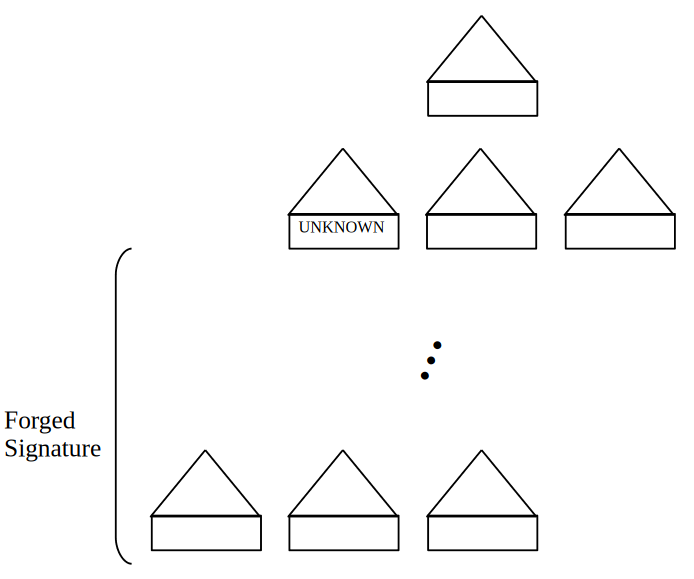
\includegraphics[width=0.5\linewidth]{fig/inter_secr_guess.png}
    \caption{Intermediate Value Guessing}
    \label{fig:intermediateValueGuessing}
\end{figure}

\subsection{Antonov's Attack}

\begin{figure}
    \centering
    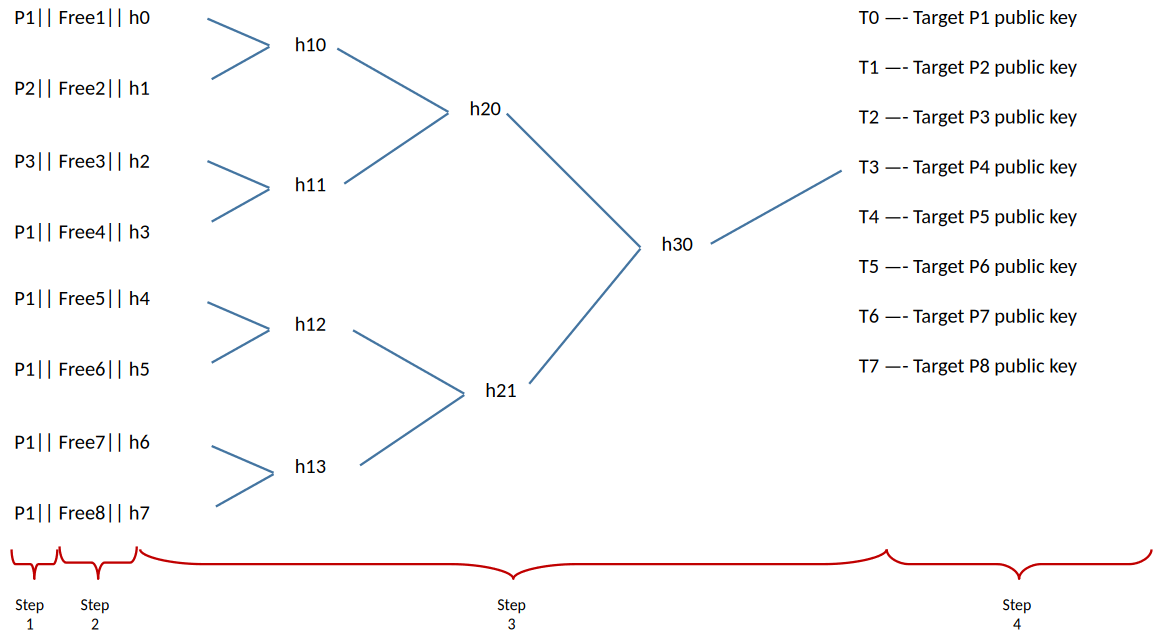
\includegraphics[width=\linewidth]{fig/antonov.png}
    \caption{Antonov's Attack}
    \label{fig:antonov}
\end{figure}

    The attack described in \cite{perlner2022breaking} exploits the Merkle–Damgård construction of the SHA-256 algorithm. Assume there are six target messages \( M_0, \ldots, M_5 \). For each message, different address values \( \text{ADRS}_0, \ldots, \text{ADRS}_5 \) are used within the hash algorithm. At this stage, intermediate values of the compression function \( C \) are obtained for each address.

Then, by applying a collision attack, the adversary finds random values \( x_0, \ldots, x_5 \), and captures pairwise collisions for the next set of intermediate values.

At this point, using the randomly found values \( X_{0,1}, X_{2,3}, X_{4,5} \), a 3-branch collision is constructed.

As the final step, the adversary finds a value \( Z \) such that the following equation holds for some \( i \in \{0,\ldots,5\} \):
\[
\text{SHA-256}(\text{ADRS}_i \,\|\, x_i \,\|\, X_{j,k} \,\|\, Z) = \text{SHA-256}(\text{ADRS}_i \,\|\, M_i)
\]

For example, if the prediction is found for \( M_3 \), then the equation
\[
\text{SHA-256}(\text{ADRS}_3 \,\|\, x_3 \,\|\, X_{2,3} \,\|\, Z) = \text{SHA-256}(\text{ADRS}_3 \,\|\, M_3)
\]
is satisfied, thus completing the multi-target prediction attack.

The complexity of finding a prediction in the final stage for \( t \) target messages is approximately \( 2^{256}/t \) compression function calls. The cost of finding an \( n \)-way collision is also determined by the number of \( C \) function evaluations.

This attack is broken down into four stages, as illustrated in Figure \ref{fig:antonov} 

\paragraph{Step 1:}
In this phase, the adversary collects a number of message-signature pairs signed using the same hash-based signature algorithm. Since the WOTS+ public keys used in the signature can be derived from the signature itself, the adversary also obtains these public keys. The attacker prefers messages with low checksum values at this stage (as lower checksums increase the probability of having \( F \) digits in the base-\( w \) representation). Although all message-signature pairs share the same \( \text{PK.seed} \), each has a distinct ADRS. In Figure~\ref{fig:collision_steps}, \( P_1, \ldots, P_8 \) represent the ADRS and PK.seed values. Finally, the attacker sorts these values.

\paragraph{Step 2:}
Here, the attacker selects random values \( \text{sk}_1, \ldots, \text{sk}_n \) and computes their hashes \( 2w \) times. By concatenating these values, they obtain the aggregated WOTS+ public keys denoted as \( \text{free}_1, \ldots, \text{free}_8 \).

\paragraph{Step 3:}
The attacker appends random values \( h \) to the free values and uses the method explained at the beginning of this section to find an \( n \)-way collision. Unlike Stage 2, the attacker does not know the secret keys corresponding to the WOTS+ public keys in this step.

\paragraph{Step 4:}
In this stage, the attacker compares the found \( n \)-way collision value with the targeted public keys using the value \( h_{30} \). \( T_0, \ldots, T_7 \) represent the target public keys before the checksum is added. If a collision is detected, the attacker has successfully forged a new WOTS+ public key whose hash value matches that of a legitimate public key.

As a result of the above steps, the attacker can generate a forged signature with a fake key. In both SPHINCS+ and XMSS algorithms, public keys generated at each layer during verification are not checked directly—instead, their hash values are computed and passed on to the next layer. Therefore, even if the attacker’s keys differ from the legitimate keys, verification succeeds as long as the hash values match. The main constraint of this attack is that the message to be signed must follow a specific format:

\begin{center}
\texttt{XXXXXXXX XXXXXXXX XXXXXXXF FFFFFFFF FFFFFFFF FFFFFFFF FFFFFFFF FFFFFFFF}
\end{center}

(where \( X \) can be any value). This requirement arises because the attacker knows the secret keys corresponding to the public keys used in Stage 2, but not those in Stage 3. In WOTS+ signatures, the public key is used to sign positions marked with \( F \); therefore, message segments where the secret key is unknown must be fixed to \( F \) to successfully carry out the attack.

\subsection{Fault Injection Attacks}

Fault injection attacks consist of scenarios in which one or more components of the algorithm are assumed to malfunction or operate incompletely due to external interference. For hash-based signature schemes, an example of a fault injection attack is described in the \cite{wagner2023faulting}.

The WOTS+ one-time signature algorithm divides the message to be signed into $w$-bit chunks and generates the signature value by repeatedly applying the hash function to the secret key as many times as the numerical value of each chunk. At this stage, an attacker can compute the hash of the signature value one more time (when the message is not $F$) to create a valid signature. To prevent this, a checksum value is appended to the message before signing. This checksum is calculated as $c = (w - 1 - m)$, where $m$ is the number of $w$-bit message chunks.

With this checksum, if the attacker computes extra hashes from the signature value, the checksum value decreases. Since the hash functions are designed to be resistant to preimage attacks, the attacker cannot compute the new checksum value. The attack described in \cite{wagner2023faulting} is based on the checksum calculation process malfunctioning due to an injected fault. If the checksum calculation does not work correctly, the attacker may generate a valid signature for a message of their choice.

\subsection{Multi-Target Attacks}

Multi-target attacks aim to find preimages when multiple output values of the used hash function are known. For a hash function with an $n$-bit output, the complexity of finding a preimage is $2^n$. In multi-target attacks, if $d$ different hash outputs are known, the complexity of finding a preimage reduces to $2^n / d$.

The XMSS and SPHINCS+ algorithms mitigate this situation by using keyed hash functions. In each usage of the hash function, different key and mask values are used, effectively differentiating the hash function for each operation and ensuring security against multi-target attacks.



\end{section}

\section{Conclusion}

Hash-based signature schemes provide a mature and theoretically sound foundation for post-quantum digital signatures. Their security is grounded in the robustness of cryptographic hash functions, making them well-suited for a future where quantum adversaries may render traditional public-key cryptosystems obsolete. 

In this paper, we presented a comprehensive overview of hash-based signature constructions, starting from early schemes like Lamport and Merkle signatures to standardized schemes such as XMSS and the stateless SPHINCS+. We analyzed their structural differences, key components, and operational procedures, including signature generation, verification, and the role of one-time signatures like WOTS and FORS. We also discussed several cryptanalytic threats specific to HBS schemes, including multi-target attacks, intermediate value recovery, and fault injection attacks, emphasizing the need for implementation-level countermeasures, especially in embedded environments.

As standardization efforts continue and implementation challenges are addressed, hash-based signature schemes are expected to play a central role in securing critical systems, firmware, and communications in the post-quantum era. Future work may focus on improving efficiency, reducing signature sizes, and designing hybrid systems that combine the strengths of HBS with other post-quantum approaches to achieve broader applicability and resilience.
